% Options for packages loaded elsewhere
\PassOptionsToPackage{unicode}{hyperref}
\PassOptionsToPackage{hyphens}{url}
%
\documentclass[
]{ltjarticle}
\usepackage{lmodern}
\usepackage{amssymb,amsmath}
\usepackage{ifxetex,ifluatex}
\ifnum 0\ifxetex 1\fi\ifluatex 1\fi=0 % if pdftex
  \usepackage[T1]{fontenc}
  \usepackage[utf8]{inputenc}
  \usepackage{textcomp} % provide euro and other symbols
\else % if luatex or xetex
  \usepackage{unicode-math}
  \defaultfontfeatures{Scale=MatchLowercase}
  \defaultfontfeatures[\rmfamily]{Ligatures=TeX,Scale=1}
\fi
% Use upquote if available, for straight quotes in verbatim environments
\IfFileExists{upquote.sty}{\usepackage{upquote}}{}
\IfFileExists{microtype.sty}{% use microtype if available
  \usepackage[]{microtype}
  \UseMicrotypeSet[protrusion]{basicmath} % disable protrusion for tt fonts
}{}
\makeatletter
\@ifundefined{KOMAClassName}{% if non-KOMA class
  \IfFileExists{parskip.sty}{%
    \usepackage{parskip}
  }{% else
    \setlength{\parindent}{0pt}
    \setlength{\parskip}{6pt plus 2pt minus 1pt}}
}{% if KOMA class
  \KOMAoptions{parskip=half}}
\makeatother
\usepackage{xcolor}
\IfFileExists{xurl.sty}{\usepackage{xurl}}{} % add URL line breaks if available
\IfFileExists{bookmark.sty}{\usepackage{bookmark}}{\usepackage{hyperref}}
\hypersetup{
  pdftitle={政府の市場介入と効率性},
  pdfauthor={アンダーランド ジェイク; 鈴鹿舞依; 白土なつき},
  hidelinks,
  pdfcreator={LaTeX via pandoc}}
\urlstyle{same} % disable monospaced font for URLs
\usepackage[top=0cm, margin=1.4cm]{geometry}
\usepackage{graphicx,grffile}
\makeatletter
\def\maxwidth{\ifdim\Gin@nat@width>\linewidth\linewidth\else\Gin@nat@width\fi}
\def\maxheight{\ifdim\Gin@nat@height>\textheight\textheight\else\Gin@nat@height\fi}
\makeatother
% Scale images if necessary, so that they will not overflow the page
% margins by default, and it is still possible to overwrite the defaults
% using explicit options in \includegraphics[width, height, ...]{}
\setkeys{Gin}{width=\maxwidth,height=\maxheight,keepaspectratio}
% Set default figure placement to htbp
\makeatletter
\def\fps@figure{htbp}
\makeatother
\setlength{\emergencystretch}{3em} % prevent overfull lines
\providecommand{\tightlist}{%
  \setlength{\itemsep}{0pt}\setlength{\parskip}{0pt}}
\setcounter{secnumdepth}{-\maxdimen} % remove section numbering
\usepackage{amsmath}
\usepackage{color}
\usepackage{hyperref}
\usepackage{luatexja}

\title{政府の市場介入と効率性}
\author{アンダーランド ジェイク \and 鈴鹿舞依 \and 白土なつき}
\date{2021-11-26}

\begin{document}
\maketitle

2021年は政府の介入のあり方が活発に議論された年だった。新型コロナウィルスの流行による消費の落ち込みは企業を切迫させ,第49回衆議院議員総選挙では補助金の支給、減税等の政府による市場介入が争点となった。岸田首相が打ち出した「新しい資本主義」は、市場介入に積極的な政府の姿勢を象徴し、従来の自民党の新自由主義路線からの差異化を図った。ただし、租税や補助金といった市場への政府の介入は、生産者価格と消費者価格の乖離を引き起こし、非効率性を生む。こうした事実を踏まえ、具体的な政府介入の例について記述した以下の文章を吟味し、正しいと思うものを1つ選びなさい。また、間違っている選択肢は、間違っている理由を説明しなさい。

\begin{enumerate}
\item 効率的な貿易政策を考える。効率性を図るための基準であるパレート最適性は次のように定義される:「誰かの状況を改善しようとすれば、他の誰かの状況を悪化させることになる」。日本では国内の米農家の利益を守るため、米に対して約800$\%$の関税を設けている。もし、この関税が撤廃されて米の自由貿易が解禁されれば、海外の低価格の米の流入により消費者は余剰を増加させるが、生産者は競走に敗退して余剰を減らしてしまう。上のパレート最適性の定義に従うと、たとえ自由貿易によって社会的余剰が増えたとしても、消費者の状況の改善が生産者の状況の悪化を意味するので、日本の現行の保護貿易政策はパレート最適であると言える。

\item 独占企業によって市場の失敗が起きている市場を考える。公正取引委員会は、この企業が独占禁止法に違反すると判断し、この法人に罰金を科した。政府は罰金で得た金額を消費者に再分配すると仮定する。これは課税ではなく、事後的な分配であるため、企業の販売戦略に影響を与えることはない。再分配の結果、生産者余剰は減り、消費者余剰が増えたので、この市場の効率性は改善された。

\item 税金は死荷重を生み、社会的余剰を減らしてしまう。しかし、税をかけても消費が減りにくい、つまり需要の価格弾力性が低い財では税金によって生じる死荷重の大きさが相対的に小さい。よって、政府の税収を確保するにあたり、生活必需品のような(需要の価格弾力性が低い)財に高い税金をかけることは社会的余剰の観点からは望ましい。一方で、消費における生活必需品の割合は、所得が低くなるほど高い。そのため、生活必需品に一律の税率を課すような税金は逆進性が高く、公平性の観点からは懸念が生じる可能性がある。


\item 特定の財の取引に際し、政府が補助金を支払うことがある。例えば、太陽光発電パネルなどの製品は、製造する企業に補助金が支払われる。これは企業の限界費用曲線、すなわち供給曲線の下降を意味する。対して、GOTOや公的住宅手当のように補助金が生産者ではなく消費者に支払われる場合は、以下のグラフのような需要曲線の上昇で表すことができる。この時、消費者余剰の\textbf{増加分}は右下のグラフの赤色の部分(CS-increase)に相当し、生産者余剰の\textbf{増加分}は右下のグラフの青色の部分(PS-increase)に相当する。死荷重は緑色の部分(DWL)に相当する。  



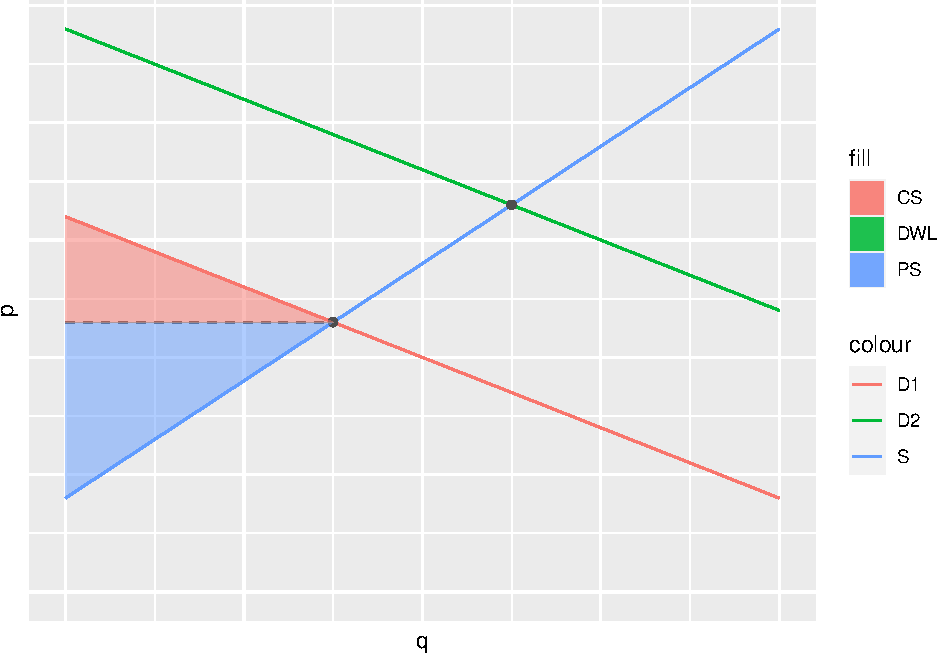
\includegraphics[width=0.5\linewidth,height=0.8\textheight]{group-report_files/figure-latex/unnamed-chunk-3-1} 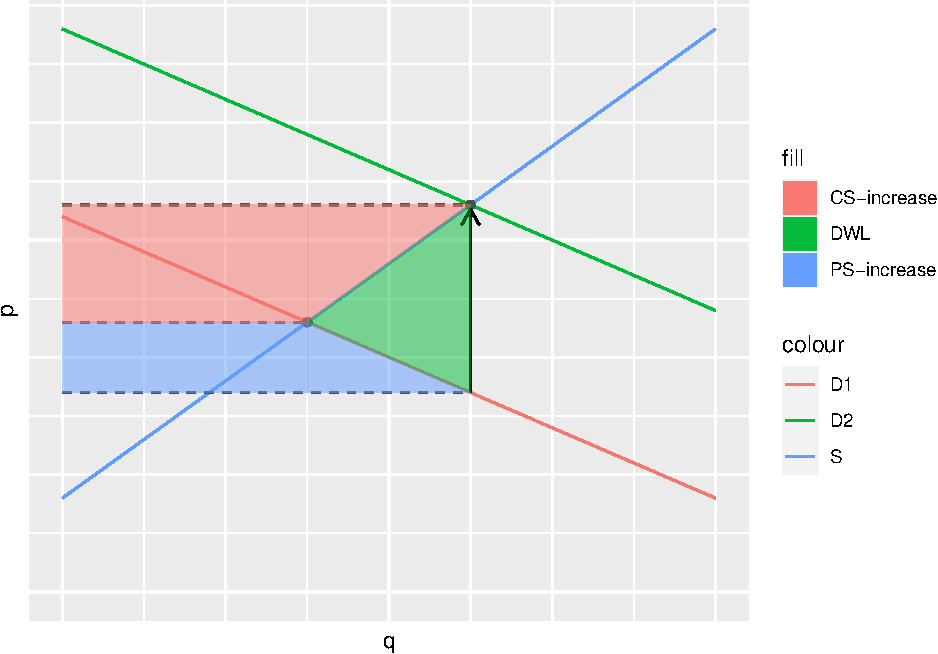
\includegraphics[width=0.5\linewidth,height=0.8\textheight]{group-report_files/figure-latex/unnamed-chunk-3-2} 


\end{enumerate}

\newpage

\hypertarget{ux6a21ux7bc4ux89e3ux7b54}{%
\section{模範解答}\label{ux6a21ux7bc4ux89e3ux7b54}}

\begin{enumerate}

\item 誤り。この場合、自由貿易によって総余剰は増加する。この時、消費者余剰を事後的に生産者に分配すれば、双方が保護貿易下に比べ余剰を増やすことができる。すると、いずれの状況を悪化させることなく、関税の撤廃と自由貿易の導入により双方の余剰を増やすことができるので、保護貿易政策はパレート効率的ではない。

\item 誤り。再分配したとしても改善されたのは公平性である。ここで行われた事後的な分配は企業の販売戦略には影響を与えない。そのため、社会的余剰の大きさは一切変わらず、その配分のみが変わるので、市場の効率性は変わらない。市場は非効率なままである。

\item 正しい。

\item 誤り。消費者余剰の増加分が青、生産者が赤であり、問題文とは逆である。正しいグラフは以下のFigure 1 に示す。ついでに、補助金が政府に支払われようが消費者に支払われようが(供給曲線の下降として表されようが需要曲線の上昇として表されようが)、それぞれの余剰の大きさ、死荷重の大きさは変わらないことが以下のFigure 1, Figure 2を比較することによってわかる。

\end{enumerate}
\begin{center} \textit{Figure 1} \end{center}

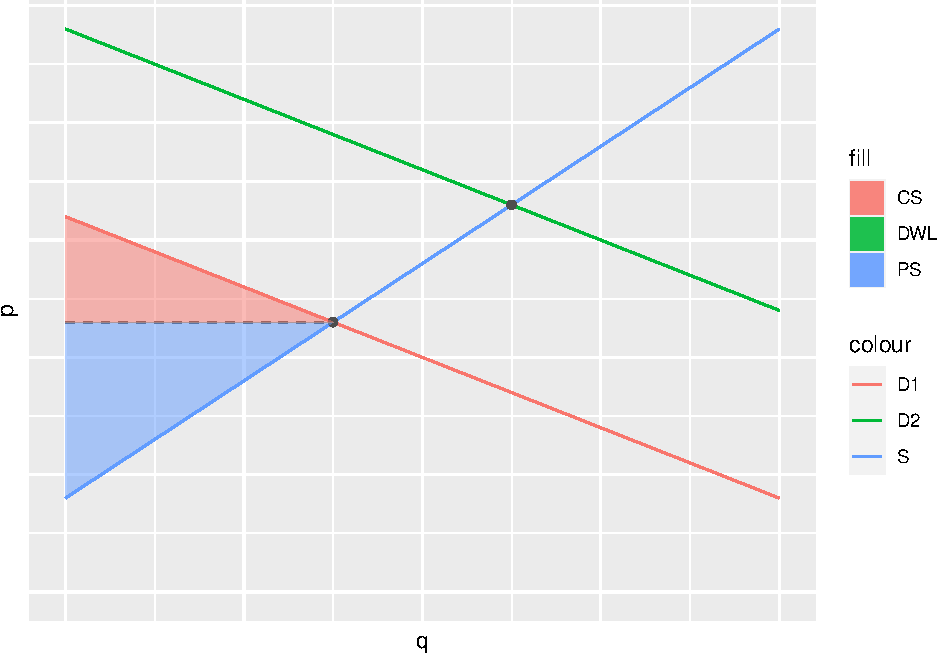
\includegraphics[width=0.5\linewidth]{group-report_files/figure-latex/version2-1}
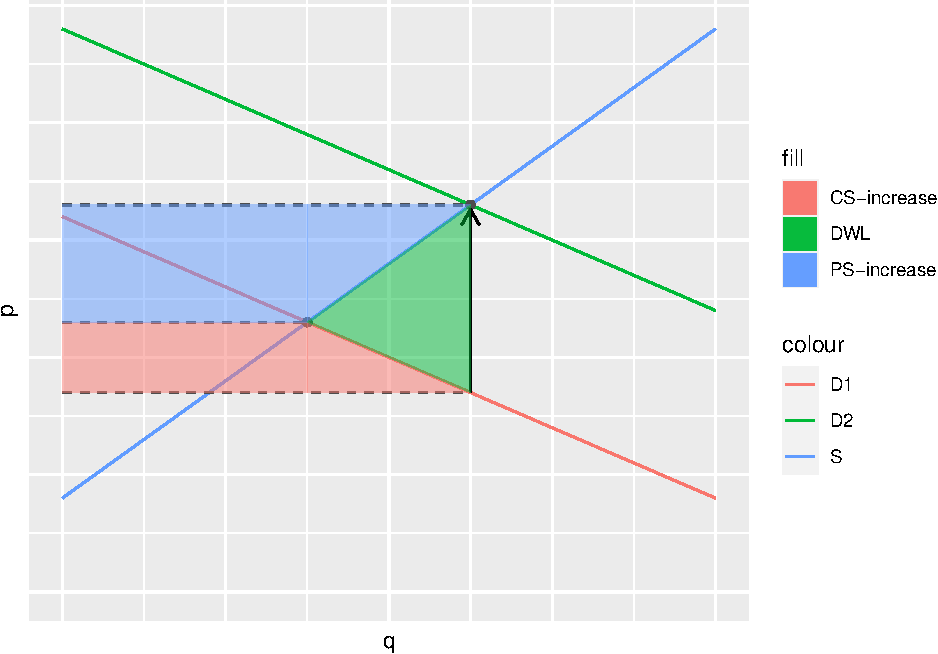
\includegraphics[width=0.5\linewidth]{group-report_files/figure-latex/version2-2}

\begin{center} \textit{Figure 2} \end{center}

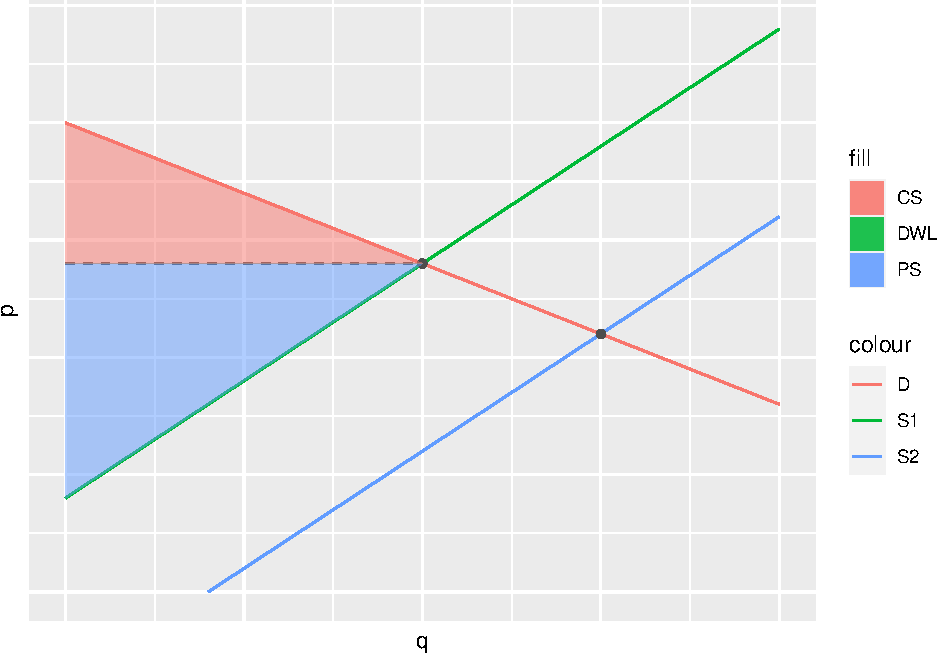
\includegraphics[width=0.5\linewidth]{group-report_files/figure-latex/version1-1}
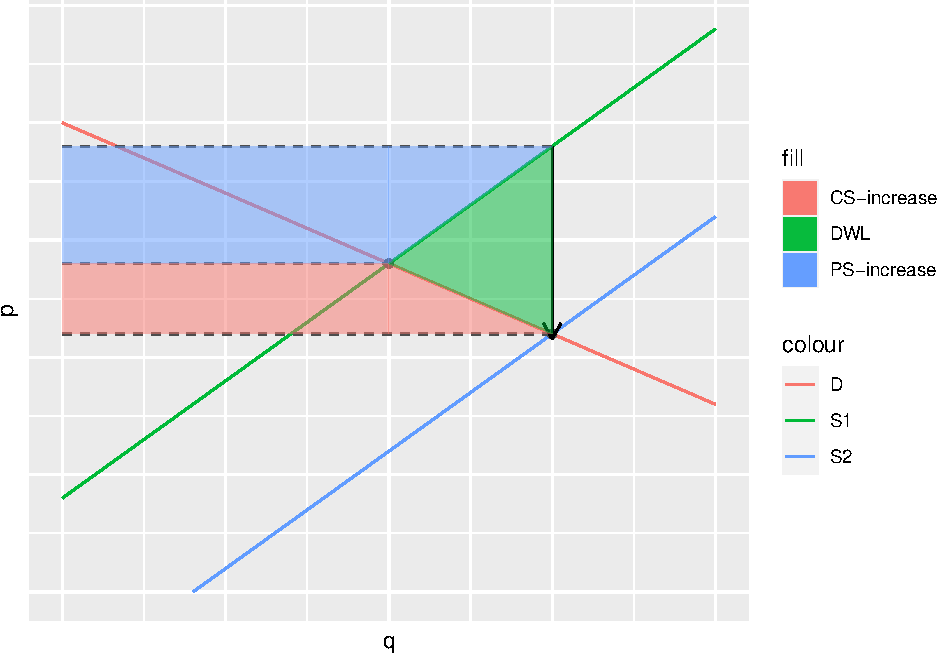
\includegraphics[width=0.5\linewidth]{group-report_files/figure-latex/version1-2}

\newpage
\newpage
\newpage

\hypertarget{paraphernalia}{%
\section{Paraphernalia}\label{paraphernalia}}

特定の財の取引に際し、政府が補助金を支払うことがある。例えば、太陽光発電パネルなどの製品は、製造する企業に補助金が支払われる。この時、左下のグラフで表されるように、企業の供給曲線(限界費用曲線)は補助金の分だけ下がり、右下のグラフに示されるような生産者余剰と消費者余剰の変化が起こる。ここで、補助金を受け取っているのは生産者なので、生産者余剰の方が大きい。対して、同じ補助金が生産者ではなく消費者に支払われる場合は、消費者の余剰の方が大きくなる。

特定の財の取引に際し、政府が補助金を支払うことがある。例えば、太陽光発電パネルなどの製品は、製造する企業に補助金が支払われる。これは企業の限界費用曲線、すなわち供給曲線の下降を意味する。対して、GOTOや公的住宅手当のように補助金が生産者ではなく消費者に支払われる場合は、以下のグラフのような需要曲線の上昇で表すことができる。この時、消費者余剰の\textbf{増加分}は右下のグラフの赤色の部分(CS-increase)に相当し、生産者余剰の\textbf{増加分}は右下のグラフの青色の部分(PS-increase)に相当する。死荷重は緑色の部分(DWL)に相当する。

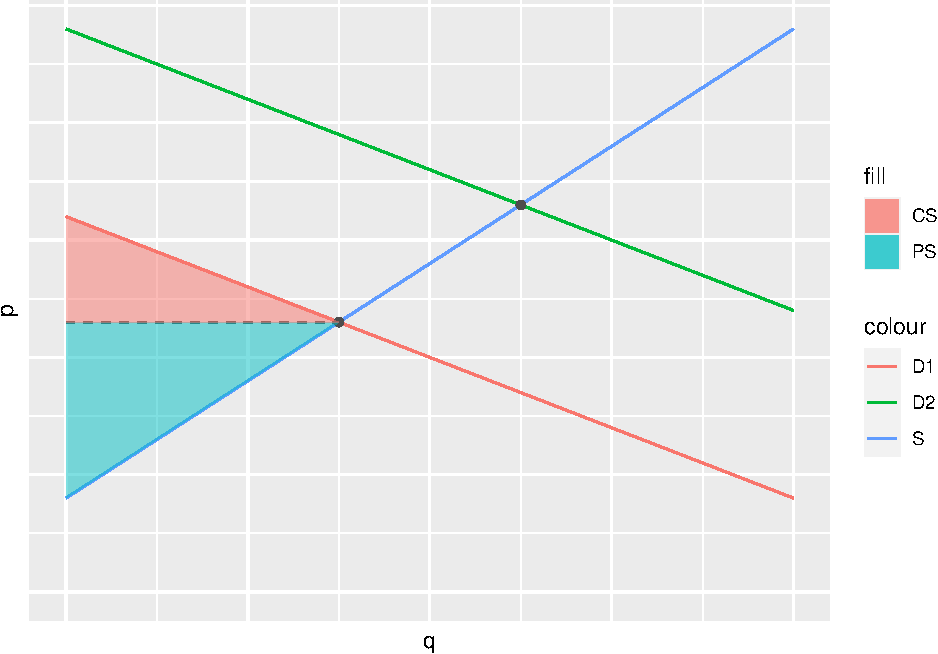
\includegraphics[width=0.5\linewidth]{group-report_files/figure-latex/unnamed-chunk-6-1}
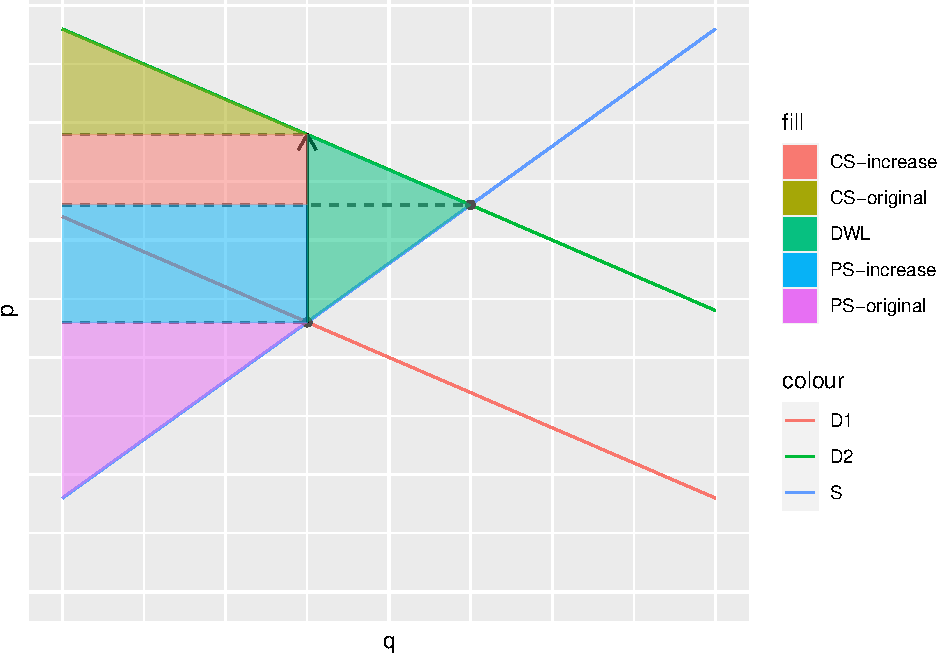
\includegraphics[width=0.5\linewidth]{group-report_files/figure-latex/unnamed-chunk-6-2}

\newpage

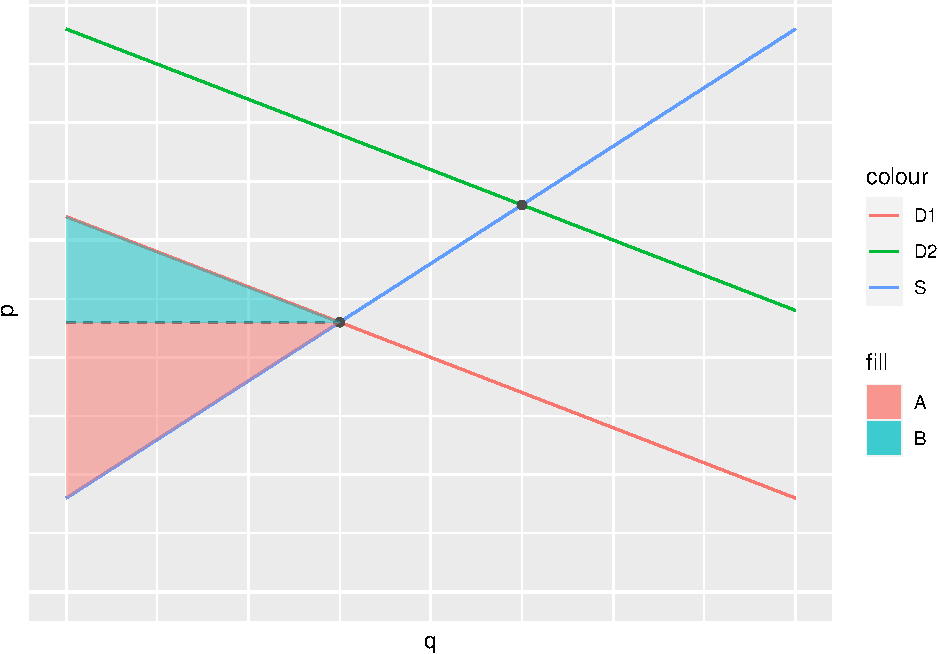
\includegraphics[width=0.5\linewidth]{group-report_files/figure-latex/version3-1}
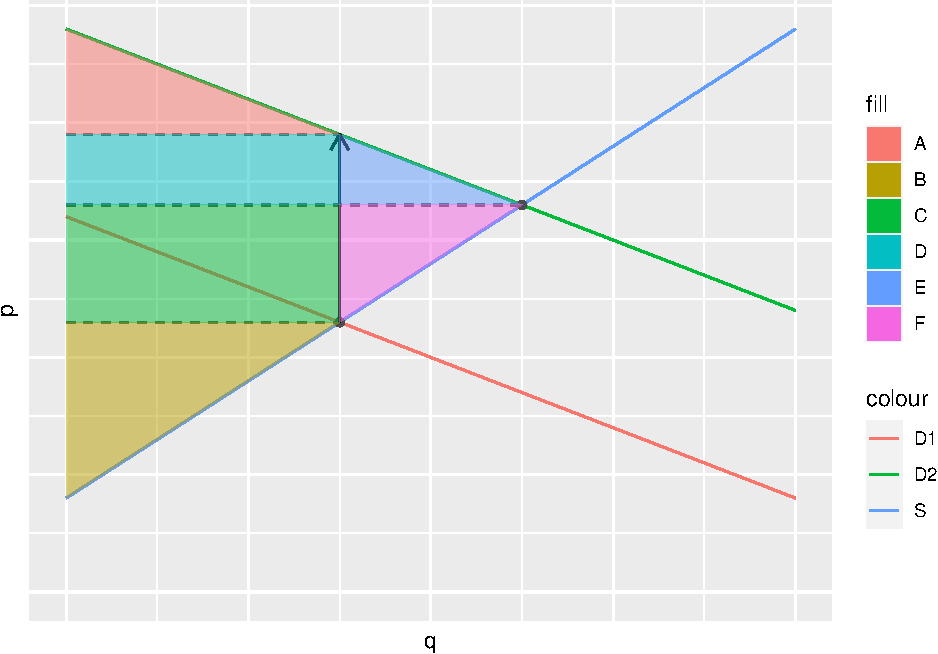
\includegraphics[width=0.5\linewidth]{group-report_files/figure-latex/version3-2}
上のグラフで補助金ありの時の消費者余剰の合計は\(A + D + E\)であり、生産者余剰の合計は\(B + C + F\)である。よって、増加分はそれぞれ\(D + E\),
\(C + F\)である。死荷重は問題文通り\(E+F\)となる。

\end{document}
